
\documentclass[border=1pt, crop, multi, tikz]{standalone} 
\usepackage{import}
\subimport{/home/thesis/PlotNeuralNets/layers/}{init}
\usetikzlibrary{positioning}
\usetikzlibrary{3d} %for including external image 

\def\ConvColor{rgb:yellow,5;red,2.5;white,5}
\def\ConvReluColor{rgb:yellow,5;red,5;white,5}
\def\PoolColor{rgb:red,1;black,0.3}
\def\UnpoolColor{rgb:blue,2;green,1;black,0.3}
\def\FcColor{rgb:blue,5;red,2.5;white,5}
\def\FcReluColor{rgb:blue,5;red,5;white,4}
\def\SoftmaxColor{rgb:magenta,5;black,7}   
\def\SumColor{rgb:blue,5;green,15}

\newcommand{\copymidarrow}{\tikz \draw[-Stealth,line width=0.8mm,draw={rgb:blue,4;red,1;green,1;black,3}] (-0.3,0) -- ++(0.3,0);}

\begin{document}
\begin{tikzpicture}
\tikzstyle{connection}=[ultra thick,every node/.style={sloped,allow upside down},draw=\edgecolor,opacity=0.7]
\tikzstyle{copyconnection}=[ultra thick,every node/.style={sloped,allow upside down},draw={rgb:blue,4;red,1;green,1;black,3},opacity=0.7]

\node[canvas is zy plane at x=0] (input) at (-3,0,0) {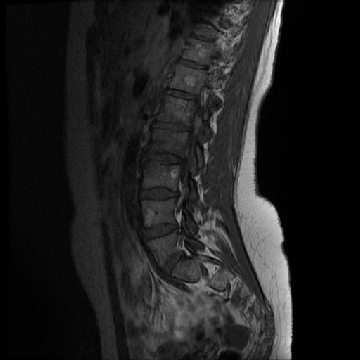
\includegraphics[width=10.0cm,height=10.0cm]{/home/thesis/PlotNeuralNets/images/input.png}};

\pic[shift={(0,0,0)}] at (0,0,0) 
    {Box={
        name=conv1,
        caption=conv1,
        xlabel={{16, }},
        zlabel=352,
        fill=\ConvColor,
        height=40,
        width=2,
        depth=40
        }
    };

\pic[shift={ (1,0,0) }] at (conv1-east) 
    {RightBandedBox={
        name=L1_1,
        caption=3x3,
        xlabel={{ 16, }},
        zlabel=352,
        fill={rgb:white,1;black,3},
        bandfill={rgb:white,1;black,2},
        opacity=0.2,
        height=40,
        width=2,
        depth=40
        }
    };

\pic[shift={(0,0,0)}] at (L1_1-east) 
    {Box={
        name=L1_2,
        caption=BN,
        xlabel={{16, }},
        zlabel=352,
        fill=\ConvColor,
        height=40,
        width=2,
        depth=40
        }
    };

\pic[shift={(1,0,0)}] at (L1_2-east) 
    {Ball={
        name=sum1,
        fill=\SumColor,
        opacity=0.6,
        radius=1.5,
        logo=$+$
        }
    };

\end{tikzpicture}
\end{document}
